\section{第四周数值分析实验}
\begin{ex}
	自行选择节点,构造插值多项式,并估计$\sqrt{2},\sqrt{2.2},\sqrt{2.5}$的值.
		不得使用牛顿切线法;不得涉及无理数运算;有效数字位数不少于$5$位.
\end{ex}
\subsection{三点三次Hermite插值}
\lstinputlisting[language=matlab]{day4/work4h33.m}
\qa [1.4142, 1.4832, 1.5811]
\subsection{两点三次Hermite插值}
\lstinputlisting[language=matlab]{day4/work4h23.m}
\qa [1.4142, 1.4833, 1.5811]
\begin{figure}[H]
	\centering
	\subfloat[三点三次Hermite插值]{\includegraphics[width = 0.5\linewidth]{day4/h33.eps}}
	\hfill
	\subfloat[两点三次Hermite插值]{\includegraphics[width = 0.5\linewidth]{day4/h23.eps}}
	\caption{运行结果}
	\label{fig:day4}
\end{figure}

